\documentclass[12pt]{article}
\usepackage[utf8]{inputenc}
\usepackage[english]{babel}
\usepackage{amsmath, amsthm, amssymb, amsfonts}
\usepackage[top = 3in, left = 1in, right = 1in]{geometry}
\usepackage{hyperref}
\hypersetup{
	colorlinks=true,
	linkcolor=blue,
	filecolor=magenta,      
	urlcolor=blue,
}
\usepackage{cleveref}
\usepackage{tcolorbox}
\usepackage{bm}

% FOR TIKZ
\usepackage{tikz}
\usetikzlibrary{arrows,arrows.meta, shapes.geometric}


% DEFINE NEW COMMANDS AND ENVIRONMENTS
\newcommand{\R}{\mathbb{R}}
\newcommand{\C}{\mathbb{C}}
\newcommand{\N}{\mathbb{N}}
\newcommand{\Q}{\mathbb{Q}}
\newcommand{\Z}{\mathbb{Z}}
\newcommand{\transpose}{\mathsf{T}}

\newcommand{\E}{\mathbb{E}}
\newcommand{\Var}{\mathbb{V}}



\newcommand{\HRule}{\rule{\linewidth}{0.5mm}} % Defines a new command for the horizontal lines, change thickness here


% DEFINE A PROBLEM Environment
\theoremstyle{definition}
\newtheorem*{prb}{Problem}
\newenvironment{problem}{
\begin{tcolorbox}[colback=blue!5!white,colframe=blue!75!black, parbox = true] \begin{prb}  }{\end{prb}\end{tcolorbox} }


\newenvironment{answer}{\textit{Solution: }\quad }{ \hfill \qedsymbol}



\begin{document}


% TITLE PAGE
%%%%%%%%%%%%%%%%%%%%%%%%%%%%%%%%%%%%%%%%%%%%%%%%%%%%%%
\begin{titlepage}
    
\centering
\textsc{\LARGE Indian Statistical Institute, Kolkata}\\[1.5cm] % Name of your university/college
\textsc{\Large Large Sample Statistical Methods}\\[0.5cm] % Major heading such as course name
% \textsc{\large Assignments in lieu of Semestral Examinations 2020}\\[0.5cm] % Minor heading such as course title

\HRule \\[0.4cm]
\large \textbf{Subhrajyoty Roy}\\
\large \textbf{Roll:  MB1911}\\
\HRule \\[1.5cm]
\normalsize \today

\end{titlepage}


\tableofcontents
\clearpage


% CONTENT FROM HERE
%%%%%%%%%%%%%%%%%%%%%%%%%%%%%%%%%%%%%%%%%%%%%%%%%%
\newgeometry{margin = 1in}

\section{Problem 1}

\begin{problem}
	Let, $F$ be a distribution function on $\R$ and $0 < p < 1$. Show that a real number $c$ is the unique quantile of order $p$ of $F$ if and only if,
	$$F(c - \epsilon) < p < F(c + \epsilon) \qquad \forall \epsilon > 0$$
\end{problem}

\begin{answer}


	\textbf{If part:}

	Here we assume, $F(c - \epsilon) < p < F(c + \epsilon)$ for any $\epsilon > 0$. Then we need to show that $c$ is the unique quantile of order $p$ of $F$.

	Taking a sequence of $\epsilon_n \rightarrow 0$, and using the above inequality for $\epsilon_n$ instead of $\epsilon$, we have;

	$$F(c-) = \lim_{n \rightarrow \infty} F(c - \epsilon_n) \leq p \leq \lim_{n \rightarrow \infty} F(c + \epsilon_n) = F(c+)$$

	However, since $F$ is a distribution function, hence it is right continuous, $F(c+) = F(c)$. This reduces to,

	$$F(c-) \leq p \leq F(c)$$

	showing that $c$ is a quantile of $F$ of order $p$. Now, to show that $c$ is the unique quantile, assume $c'$ is another quantile of $F$ of order $p$. Then we have by definition of quantile,

	\begin{equation}
		F(c'-) \leq p \leq F(c')
		\label{eqn:1-1}
	\end{equation}

	If $c > c'$, then $\epsilon = (c - c') > 0$, and by the given condition $F(c') = F(c - \epsilon) < p$ which contradicts \eqref{eqn:1-1}. On the other hand, if $c' > c$, then $\epsilon = (c' - c) > 0$. Then again by the given condition, $F(c' - \epsilon/2) = F(c + \epsilon/2) > p$, but since $F(c'-) \leq p$, it must be the case that $F(c' - \epsilon/2) \leq F(c'-) \leq p$, leading to another contradiction.

	\textbf{Only if part:}
	Now, we assume that $c$ is the unique quantile of order $p$ of $F$, and we need to show that for any given $\epsilon > 0$, we have; $F(c - \epsilon) < p < F(c + \epsilon)$.

	Now since $c$ is a $p$-th quantile, by definition we have $F(c-) \leq p \leq F(c)$. Also, since $F$ is non-decreasing, we have for any given $\epsilon > 0$, $F(c-\epsilon) \leq F(c-) \leq p \leq F(c) \leq F(c+\epsilon)$. We simply need to show that it holds with a strict inequality.

	Let us assume otherwise. Then we consider two cases.

	\begin{enumerate}
		\item First case is that for some $\epsilon_0 > 0$, $F(c - \epsilon_0) = p$. Then clearly, $F((c - \epsilon_0) - ) \leq p \leq F(c - \epsilon_0)$, therefore, showing that $(c - \epsilon_0)$ is also a $p$-th order quantile. But, as $\epsilon_0 > 0$, $c \neq (c - \epsilon_0)$, contradicting the assumption that $c$ is the unique $p$-th quantile.
		\item For the second case, assume for some $\epsilon_0 > 0$, $F(c + \epsilon_0) = p$. Then again by exactly same logic, $(c + \epsilon_0)$ is another $p$-th quantile, contradicting to the uniqueness of $c$.
	\end{enumerate}

	Therefore, we must have, $F(c -\epsilon) < p < F(c+ \epsilon)$ for any $\epsilon > 0$, completing the proof.

\end{answer}


\section{Problem 2}

\begin{problem}
	Let, $X_1, X_2, \dots X_n$ be a random sample from a distribution symmetric about $0$, and having finite $8$-th moment. Find the asymptotic distribution of the following measures of skewness and kurtosis:

	\begin{enumerate}
		\item[(a)] $g_{1n} = \dfrac{m_{3n}}{m_{2n}^{3/2}}$
		\item[(b)] $g_{2n} = \dfrac{m_{4n}}{m_{2n}^2} - 3$ 
	\end{enumerate}

	where $m_{rn}$ is the $r$-th order sample central moment. First find the result for the general case and then use it to derive for the case when the underlying distribution is $N(\mu, \sigma^2)$. 
\end{problem}

\begin{answer}
	By a simple application of multivariate central limit theorem for $X_1, X_2, \dots X_n$, and using \textbf{Theorem D} (in the section related to asymptotic distribution of moments), we have $\sqrt{n} (T_n - \bm{\mu})$ is asymptotically normal with mean parameter $\bm{0}$ and dispersion matrix $\Sigma = ((\sigma_{ij}))$, where;

	$$T_n = \begin{bmatrix}
		m_{1n}\\
		m_{2n}\\
		m_{3n}\\
		m_{4n}\\
	\end{bmatrix} \quad \text{ and } \quad 
	\bm{\mu} = \begin{bmatrix}
		\mu_1\\
		\mu_2\\
		\mu_3\\
		\mu_4\\
	\end{bmatrix}
	$$

	and 
	
	$$
	\sigma_{ij} = \mu_{i+j} - \mu_i \mu_j - i\mu_{i-1}\mu_{i+1} - j\mu_{j-1}\mu_{j+1} + ij \mu_{i-1}\mu_{j-1}\mu_2
	$$


	where $m_{rn}$ is the $r$-th order sample central moment and $\mu_r$ is the $r$-th order population central moment.

	Now, since $X_1, X_2, \dots X_n$ is a random sample from a distribution symmetric about $0$, clearly, all odd order population central moments will be equal to $0$, i.e. $\mu_1 = \mu_3 = 0$. Therefore, $\bm{\mu} = (0, \mu_2, 0, \mu_4)^T$
	Also, let us denote the set of permissible values for the vector $T_n$ as $A$, i.e.

	$$A = \left\{ (x_1,x_2,x_3, x_4) : x_i \in \R \quad \forall i = 1, 2, 3, 4 \text{ and } x_2 \geq 0, x_4 \geq 0 \right\}$$

	\begin{enumerate}
		\item[(a)]  Consider the function, $g : A \rightarrow \R$ given by;
		$$g(x_1, x_2, x_3, x_4) = \dfrac{x_3}{x_2^{3/2}}$$
		
		\begin{align*}
			\therefore \quad 
			& \nabla g(\bm{x}) = \left( 0, -\dfrac{3}{2} \dfrac{x_3}{x_2^{5/2}}, \dfrac{1}{x_2^{3/2}}, 0 \right)\\
			\Rightarrow \quad & \nabla g(\bm{\mu}) = \left( 0, 0, \mu_2^{-3/2}, 0 \right)
		\end{align*}

		Now, applying delta method, we get that, $\sqrt{n}(g(T_n) - g(\bm{\mu}))$ is asymptotically normal with mean $\bm{0}$ and dispersion $\nabla g(\bm{\mu})^T \Sigma \nabla g(\bm{\mu})$. But note that, $g(T_n) = g_{1n}$ and $g(\bm{\mu}) = \dfrac{\mu_3}{\mu_2^{3/2}} = 0$. And finally,

		\begin{align*}
			\nabla g(\bm{\mu})^T \Sigma \nabla g(\bm{\mu})
			& = \dfrac{1}{\mu_2^3} \sigma_{33}\\
			& = \dfrac{1}{\mu_2^3} \left( \mu_6 - \mu_3^2 - 6\mu_2\mu_4 + 9\mu_2^3 \right)\\
			& = \dfrac{1}{\mu_2^3} \left( \mu_6 - 6\mu_2\mu_4 + 9\mu_2^3 \right)\\
			& = \dfrac{\mu_6}{\mu_2^3} - 6\dfrac{\mu_4}{\mu_2^2} + 9
		\end{align*}

		So, we have;

		$$\sqrt{n} g_{1n} \text{ is Asymptotically Normal} \left(0, \dfrac{\mu_6}{\mu_2^3} - 6\dfrac{\mu_4}{\mu_2^2} + 9 \right)$$
		

		In case the samples $X_1, X_2, \dots X_n$ comes from a normal distribution with parameters $\mu$ and $\sigma^2$, we consider the standardized samples, $Z_i = \dfrac{(X_i - \mu)}{\sigma}$. Then, $Z_1, Z_2, \dots Z_n \sim N(0, 1)$ and more importantly, the sample and population skewness and kurtosis coefficients of $X_i$'s and $Z_i$'s are same. Hence, it is enough to consider $Z_i$'s instead $X_i$'s, i.e. the underlying distribution being the standard normal distribution and the same asymptotic distribution can be applied in any $N(\mu, \sigma^2)$ distribution for any $\mu \in \R$ and $\sigma^2 > 0$.
		
		Considering standard normal distribution, we have;

		$$\mu_{2k} = (2k-1)(2k-3)\dots 3.1 \qquad \forall k \in \N$$

		Using this, we get $\mu_6 = 15, \mu_4 = 3, \mu_2 = 1$, and hence, $\dfrac{\mu_6}{\mu_2^3} - 6\dfrac{\mu_4}{\mu_2^2} + 9 = (15 - 18 + 9) = 6$. Therefore, in case the underlying distribution is a normal distribution,
		
		$$\sqrt{n} g_{1n} \text{ is Asymptotically Normal} \left(0, 6 \right)$$
		

		\item[(b)]  For this case, consider the function, $h : A \rightarrow \R$ given by;
		$$h(x_1, x_2, x_3, x_4) = \dfrac{x_4}{x_2^2} - 3$$
		
		\begin{align*}
			\therefore \quad 
			& \nabla h(\bm{x}) = \left( 0, -2 \dfrac{x_4}{x_2^3}, 0, \dfrac{1}{x_2^2} \right)\\
			\Rightarrow \quad & \nabla h(\bm{\mu}) = \left( 0, -2 \dfrac{\mu_4}{\mu_2^3}, 0, \dfrac{1}{\mu_2^2} \right)
		\end{align*}

		Now, applying delta method, we get that, $\sqrt{n}(h(T_n) - h(\bm{\mu}))$ is asymptotically normal with mean $\bm{0}$ and dispersion $\nabla h(\bm{\mu})^T \Sigma \nabla h(\bm{\mu})$. But note that, $h(T_n) = g_{2n}$ and $h(\bm{\mu}) = \dfrac{\mu_4}{\mu_2^2} - 3$, the population coefficient of kurtosis. Hence,

		\begin{align*}
			\nabla h(\bm{\mu})^T \Sigma \nabla h(\bm{\mu})
			& = 4 \dfrac{\mu_4^2}{\mu_2^6} \sigma_{22} - 4 \dfrac{\mu_4}{\mu_2^5}\sigma_{24} + \dfrac{1}{\mu_2^2} \sigma_{44}\\
			& = 4 \dfrac{\mu_4^2}{\mu_2^6} \left[ \mu_4 - \mu_2^2 - 4 \mu_1\mu_3 + 4 \mu_1^2 \mu_2 \right] - 4 \dfrac{\mu_4}{\mu_2^5} \left[ \mu_6 - \mu_2\mu_4 - 2\mu_1\mu_3 - 4\mu_3\mu_5 + 8 \mu_1\mu_3\mu_2 \right]\\
			& \qquad \qquad + \dfrac{1}{\mu_2^2} \left[ \mu_8 - \mu_4^2 - 8 \mu_3 \mu_5 + 16 \mu_3^2\mu_2 \right]\\
			& = 4 \dfrac{\mu_4^2}{\mu_2^6} \left( \mu_4 - \mu_2^2 \right) - 4 \dfrac{\mu_4}{\mu_2^5} \left( \mu_6 - \mu_2\mu_4 \right) + \dfrac{1}{\mu_2^2} \left( \mu_8 - \mu_4^2 \right)\\
		\end{align*}

		Therefore, again by application of delta method, we simply have,

		$$\sqrt{n} (g_{2n} - \kappa) \text{ is Asymptotically Normal} \left(0, 4 \dfrac{\mu_4^2}{\mu_2^6} \left( \mu_4 - \mu_2^2 \right) - 4 \dfrac{\mu_4}{\mu_2^5} \left( \mu_6 - \mu_2\mu_4 \right) + \dfrac{1}{\mu_2^2} \left( \mu_8 - \mu_4^2 \right) \right)$$

		where $\kappa = \dfrac{\mu_4}{\mu_2^2} - 3$, the population coefficient of kurtosis.
		
		In case the underlying distribution of the samples is standard normal distribution, using $\mu_8 = (7\times 5 \times 3) = 105, \mu_6 = 15, \mu_4 = 3$ and $\mu_2 = 1$, and noting that $\kappa = 0$, we have;

		\begin{align*}
			& 4 \dfrac{\mu_4^2}{\mu_2^6} \left( \mu_4 - \mu_2^2 \right) - 4 \dfrac{\mu_4}{\mu_2^5} \left( \mu_6 - \mu_2\mu_4 \right) + \dfrac{1}{\mu_2^2} \left( \mu_8 - \mu_4^2 \right)\\
			= \quad & 4 \times 3^2 \times (3 - 1^2) - 4 \times 3 \times (15 - 3) + (105 - 3^2)\\
			= \quad & 72 - 144 + 105 - 9 = 24\\
		\end{align*}

		i.e. for the case where underlying distribution is a normal distribution (or standard normal distribution, since similar to previous logic we can consider $Z_i$'s here),

		$$\sqrt{n} g_{2n} \text{ is Asymptotically Normal} \left(0, 24 \right)$$
	\end{enumerate}

\end{answer}


\section{Problem 3}
\begin{problem}
	Let, $X_1, X_2, \dots X_n$ be i.i.d $N(\theta, 1)$ variables where it is known that $\vert \theta \vert \leq 1$. Find the mle of $\theta$ and also find its asymptotic distribution under any $\theta_0 \in (-1, 1)$.
\end{problem}

\begin{answer}
	We are given, $X_i \sim N(\theta, 1)$ be iid random variables, $i = 1, 2, \dots n$. Therefore, the likelihood function upto a constant multiple is given as;

	\begin{equation}
		\mathcal{L}(\theta) \propto \exp\left\{ -\dfrac{1}{2} \sum_{i=1}^{n} (X_i - \theta)^2 \right\} \bm{1}_{\vert \theta \vert \leq 1}
	\end{equation}

	Now to find the maximizer of the likelihood function $\mathcal{L}(\theta)$, letting $\overline{X}_n$ as the sample mean based on $X_1, X_2, \dots X_n$, consider the following;

	\begin{align*}
		& \mathcal{L}(\theta) \propto \exp\left\{ -\dfrac{1}{2} \sum_{i=1}^{n} (X_i - \overline{X}_n + \overline{X}_n - \theta)^2 \right\} \bm{1}_{\vert \theta \vert \leq 1}\\
		\Rightarrow \quad & \mathcal{L}(\theta) \propto \exp\left\{ -\dfrac{1}{2} \left[\sum_{i=1}^{n} (X_i - \overline{X}_n)^2 + n(\overline{X}_n - \theta)^2 \right] \right\} \bm{1}_{\vert \theta \vert \leq 1}\\
		\Rightarrow \quad & \mathcal{L}(\theta) \propto \exp\left\{ -\dfrac{n}{2} (\overline{X}_n - \theta)^2 \right\} \bm{1}_{\vert \theta \vert \leq 1}\\
	\end{align*}

	Clearly, this likelihood as a function of $\theta$ decreases to both side of $\overline{X}_n$ as $\vert \overline{X}_n - \theta \vert$ increases in magnitude, and if $\theta$ lies outside the interval $[-1, 1]$, the likelihood function becomes $0$.

	Hence, the likelihood function is maximized at $\theta = \overline{X}_n$, if $\overline{X}_n \in [-1, 1]$, and otherwise, the maximization happens at the endpoint of the interval $[-1, 1]$ which is closest to $\overline{X}_n$. Therefore, the mle of $\theta$ is;

	$$
	\widehat{\theta}_n = \begin{cases}
		\overline{X}_n & \text{ if } (-1) \leq \overline{X}_n \leq 1\\
		1 & \text{ if } \overline{X}_n > 1\\
		(-1) & \text{ if } \overline{X}_n < (-1)\\
	\end{cases}
	$$

	Now, to find the asymptotic distribution of $\widehat{\theta}_n$, we consider the following quantity;

	\begin{align*}
		& P_{\theta_0} \left( \sqrt{n}(\widehat{\theta}_n - \theta_0) \leq x \right)\\
		= \quad & P_{\theta_0} \left( \sqrt{n}(\widehat{\theta}_n - \theta_0) \leq x, \overline{X}_n \in (-1, 1) \right) + P_{\theta_0} \left( \sqrt{n}(\widehat{\theta}_n - \theta_0) \leq x , \overline{X}_n \geq 1\right) \\
		& \qquad + P_{\theta_0} \left( \sqrt{n}(\widehat{\theta}_n - \theta_0) \leq x, \overline{X}_n \leq (-1) \right)\\
		= \quad & P_{\theta_0} \left( \sqrt{n}(\overline{X}_n - \theta_0) \leq x \right)P_{\theta_0} \left( \overline{X}_n \in (-1, 1) \right) + P_{\theta_0} \left( \sqrt{n}(\delta_{1} - \theta_0) \leq x \right)P_{\theta_0} \left( \overline{X}_n \geq 1 \right) \\
		& \qquad + P_{\theta_0} \left( \sqrt{n}(\delta_{-1} - \theta_0) \leq x \right)P_{\theta_0} \left( \overline{X}_n \leq (-1) \right)
	\end{align*}

	where $\delta_x$ is the degenerate distribution at $x$. Now note that, $\overline{X}_n \sim N(\theta_0, \dfrac{1}{n})$ under $\theta_0$ being the true parameter. Therefore,

	$$
	\begin{array}{l}
		P_{\theta_0}\left( \overline{X}_n < 1 \right) = \Phi\left( \sqrt{n}(1-\theta_0) \right)\\
		P_{\theta_0}\left( \overline{X}_n < (-1) \right) = \Phi\left( \sqrt{n}(-1-\theta_0) \right)\\
	\end{array}
	$$

	where $\Phi(\cdot)$ is the cumulative distribution function of standard normal distribution. Also note that, since the true parameter $\theta_0 \in (-1, 1)$, $(1 - \theta_0) > 0$ and $(-1 - \theta_0) < 0$. Hence, as $n \rightarrow \infty$,

	$$
	\begin{array}{l}
		\sqrt{n}(1 - \theta_0) \rightarrow \infty\\
		\sqrt{n}(-1 - \theta_0) \rightarrow -\infty\\
	\end{array}
	$$

	Hence, for sufficiently large $n$, i.e. for any $n \geq N =  \max\left\{ \dfrac{x^2}{(1-\theta_0)^2}, \dfrac{x^2}{(-1-\theta_0)^2} \right\}$, we have;

	$$
	\begin{array}{l}
		P_{\theta_0}(\sqrt{n}(\delta_1 - \theta_0) \leq x) = 0\\
		P_{\theta_0}(\sqrt{n}(\delta_{-1} - \theta_0) \leq x) = 1\\
	\end{array}
	$$

	Hence for any $n \geq N$, we have;

	$$
	P_{\theta_0} \left( \sqrt{n}(\widehat{\theta}_n - \theta_0) \leq x \right) = \Phi(x) \left[ \Phi\left( \sqrt{n}(1-\theta_0) \right) - \Phi\left( \sqrt{n}(-1-\theta_0) \right) \right] + \Phi\left( \sqrt{n}(-1-\theta_0) \right)
	$$

	Now taking limit as $n \rightarrow \infty$, we obtain;

	\begin{align*}
		& P_{\theta_0} \left( \sqrt{n}(\widehat{\theta}_n - \theta_0) \leq x \right)\\
		= \quad & \Phi(x) \left[ \Phi\left( \sqrt{n}(1-\theta_0) \right) - \Phi\left( \sqrt{n}(-1-\theta_0) \right) \right] + \Phi\left( \sqrt{n}(-1-\theta_0) \right)\\
		\xrightarrow{n \rightarrow \infty} \quad & \Phi(x) \left[ \Phi\left( \infty \right) - \Phi\left( -\infty \right) \right] + \Phi\left( -\infty \right)\\
		= \quad & \Phi(x)
	\end{align*}

	Therefore, for all $x \in \R = \mathcal{C}(\Phi)$, i.e. the continuity points of $\Phi(\cdot)$, the distribution function of $\sqrt{n}(\widehat{\theta}_n - \theta_0)$ converges to the distribution function of standard normal distribution, i.e. we have,

	$$\sqrt{n}(\widehat{\theta}_n - \theta_0) \xrightarrow{d} Z \sim N(0, 1)$$

	i.e. the suitably centered and scaled random variable of the MLE, $\sqrt{n}(\widehat{\theta}_n - \theta_0)$ follows an asymptotic normal distribution with mean $0$ and variance $1$.
\end{answer}


\section{Problem 4}
\begin{problem}
	Let, $X_1, X_2, \dots X_n$ be a random sample from a distribution with a density $f(x \mid \theta), \theta \in \Theta$, an open interval in $\R$. Assume suitable regularity conditions on the densities so that there is a consistent solution $\widehat{\theta}_n$ of the likelihood equation for which $\sqrt{n}(\widehat{\theta}_n - \theta)$ is $AN(0, \mathcal{I}^{-1}(\theta))$, under $\theta$. Fix, $\theta_0 \in \Theta$ and set,
	
	$$T_n = \begin{cases}
		\widehat{\theta}_n & \text{ if } \vert \widehat{\theta}_n - \theta_0 \vert > n^{-1/4}\\
		\theta_0 & \text{ if } \vert \widehat{\theta}_n - \theta_0 \vert \leq n^{-1/4}\\
	\end{cases}$$

	Find the asymptotic distribution of $\sqrt{n}(T_n - \theta)$ under $\theta$. 
\end{problem}


\begin{answer}
	We shall consider two separate cases, where true $\theta = \theta_0$ and another case where $\theta \neq \theta_0$.
	
	\textbf{Case 1:} $\theta \neq \theta_0$.

	Consider the quantity, $Z_n = \sqrt{n} (T_n - \widehat{\theta}_n)$. Note that,

	$$
	Z_n = \begin{cases}
		0 & \text{ if } \vert \widehat{\theta}_n - \theta_0 \vert > n^{-1/4}\\
		\sqrt{n} (\theta_0 - \widehat{\theta}_n) & \text{ if } \vert \widehat{\theta}_n - \theta_0 \vert \leq n^{-1/4}
	\end{cases}
	$$

	Therefore,

	\begin{align*}
		P_{\theta} (Z_n \neq 0) 
		& \leq P_{\theta} \left( \vert \widehat{\theta}_n - \theta_0 \vert \leq n^{-1/4} \right)\\
		& = P_{\theta} \left( \widehat{\theta}_n \geq \theta_0 - n^{-1/4}, \widehat{\theta}_n \leq \theta_0 + n^{-1/4} \right)\\
		& = P_{\theta} \left( (\widehat{\theta}_n - \theta) \geq (\theta_0 - \theta) - n^{-1/4}, (\widehat{\theta}_n - \theta) \leq (\theta_0 - \theta) + n^{-1/4} \right)
	\end{align*}

	Now, if $\theta_0 > \theta$, then for sufficiently large $n$, we have, $(\theta_0 - \theta) - n^{-1/4} > \epsilon > 0$ for some $\epsilon > 0$. Hence in this case,

	\begin{align*}
		P_{\theta} (Z_n \neq 0) 
		& \leq P_{\theta} \left( (\widehat{\theta}_n - \theta) \geq (\theta_0 - \theta) - n^{-1/4} \right)\\
		& \leq P_{\theta} \left( (\widehat{\theta}_n - \theta) \geq \epsilon \right)\\
		& \qquad \text{ for sufficently large } n \text{ as, }\\
		& \qquad (\widehat{\theta}_n - \theta) \geq ((\theta_0 - \theta) - n^{-1/4}) \implies (\widehat{\theta}_n - \theta) \geq \epsilon\\
		& \leq P_{\theta} \left(\vert \widehat{\theta}_n - \theta \vert \geq \epsilon \right)\\
		& \qquad \text{since, } (\widehat{\theta}_n - \theta) \geq \epsilon \implies \vert \widehat{\theta}_n - \theta \vert \geq \epsilon\\
		& \rightarrow 0 \qquad \text{since, } \widehat{\theta}_n \xrightarrow{P} \theta
	\end{align*}

	If $\theta_0 < \theta$, then similarly, for sufficiently large $n$, we have $(\theta_0 - \theta) + n^{-1/4} < -\epsilon < 0$, for some $\epsilon > 0$. Therefore,

	\begin{align*}
		P_{\theta} (Z_n \neq 0) 
		& \leq P_{\theta} \left( (\widehat{\theta}_n - \theta) \leq (\theta_0 - \theta) + n^{-1/4} \right)\\
		& \leq P_{\theta} \left( (\widehat{\theta}_n - \theta) \leq -\epsilon \right)\\
		& \qquad \text{ for sufficently large } n \text{ as, }\\
		& \qquad (\widehat{\theta}_n - \theta) \leq ((\theta_0 - \theta) + n^{-1/4}) \implies (\widehat{\theta}_n - \theta) \leq (-\epsilon)\\
		& \leq P_{\theta} \left(\vert \widehat{\theta}_n - \theta \vert \geq \epsilon \right)\\
		& \qquad \text{since, } (\widehat{\theta}_n - \theta) \leq (-\epsilon) \implies \vert \widehat{\theta}_n - \theta \vert \geq \epsilon\\
		& \rightarrow 0 \qquad \text{since, } \widehat{\theta}_n \xrightarrow{P} \theta
	\end{align*}

	Hence we have, $P_{\theta}(Z_n \neq 0) \rightarrow 0$, and hence, by definition of convergence in probability, $Z_n \xrightarrow{P} 0$ under $\theta$. 
	
	Now, we know that, $\sqrt{n}(\widehat{\theta}_n - \theta) \xrightarrow{d} N(0, \mathcal{I}^{-1}(\theta))$, and $Z_n = \sqrt{n}(T_n - \widehat{\theta}_n) \xrightarrow{P} 0$. Therefore, an application of Slutsky's theorem yields,

	\begin{equation}
		\sqrt{n}(T_n - \theta) = \sqrt{n}(\widehat{\theta}_n - \theta) + Z_n \xrightarrow{d} N(0, \mathcal{I}^{-1}(\theta))
		\label{eqn:4-case1}
	\end{equation}


	\textbf{Case 2: } Now we proceed to the case where $\theta = \theta_0$. In this case, consider the random variable,

	$$\sqrt{n}(T_n - \theta_0) = \begin{cases}
		\sqrt{n} (\widehat{\theta}_n - \theta_0) & \text{ if } \vert \widehat{\theta}_n - \theta_0 \vert > n^{-1/4}\\
		0 & \text{ if } \vert \widehat{\theta}_n - \theta_0 \vert \leq n^{-1/4}\\
	\end{cases}
	$$

	Similar to before, consider the following probability under $\theta = \theta_0$;

	\begin{align*}
		P_{\theta_0} \left( \sqrt{n}(T_n - \theta_0) \neq 0 \right)
		& \leq P_{\theta_0} \left( \vert \widehat{\theta}_n - \theta_0 \vert > n^{-1/4} \right)\\
		& = P_{\theta_0} \left( \vert \sqrt{n} (\widehat{\theta}_n - \theta_0) \vert > n^{1/4} \right)\\
		& \leq \dfrac{\text{Var}_{\theta_0} (\widehat{\theta}_n)}{\sqrt{n}} \quad \text{, by Chebyshev's inequality}\\
		& = \dfrac{\mathcal{I}^{-1}(\theta_0) }{\sqrt{n}}\\
		& \xrightarrow{n \rightarrow \infty} 0
	\end{align*}

	Hence, if $\theta = \theta_0$, then under $\theta = \theta_0$, $\sqrt{n}(T_n - \theta_0) \xrightarrow{P} 0$, and as in probability convergence implies convergence in distribution, we have;

	\begin{equation}
		\sqrt{n}(T_n - \theta_0) \xrightarrow{d} \delta_0\\
		\label{eqn:4-case2}
	\end{equation}

	where $\delta_x$ is the distribution degenerate at $x$.

	Thus, combining the equations \eqref{eqn:4-case1} and \eqref{eqn:4-case2}, we obtain that under any $\theta \in \Theta$, the quantity $\sqrt{n}(T_n - \theta)$ follows an asymptotic normal distribution with mean $0$ and variance $v(\theta)$, where $v(\theta)$ is given by;

	$$
	v(\theta) = \begin{cases}
		\mathcal{I}^{-1}(\theta) & \text{ if } \theta \neq \theta_0\\
		0 & \text{ if } \theta = \theta_0
	\end{cases}
	$$

	where the normal distribution with mean $0$ and variance $0$ is another notion of specifying the distribution degenerate at $0$.

\end{answer}


\vspace*{1in}

\begin{center}
	{\Large\textit{Thank you}}
	\vspace*{0.25in}\\
	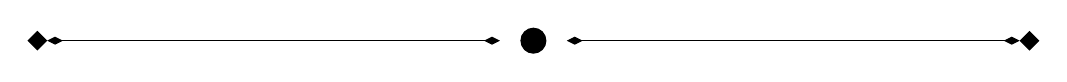
\begin{tikzpicture}[scale = 3]
		\node (a) at (0,0) {};
		\node (b) at (2,0) {};
		\draw[fill] (2.1, 0) circle (1.5pt);
		\node[draw, diamond, fill = black, scale = 0.5] at (0,0) {};
		\node (d) at (2.2,0) {};
		\node (e) at (4.2,0) {};
		\node[draw, diamond, fill = black, scale = 0.5] at (4.2,0) {};
		\draw [{Diamond}-{Diamond}] (a.east) -- (b.west);
		\draw [{Diamond}-{Diamond}] (d.east) -- (e.west);
	\end{tikzpicture}
\end{center}



\end{document}

